\section {ECN versus Delay}
\label{sec:discuss}
In the previous sections, we saw that barring the small anomaly, DCQCN remains
stable as the number of flows increase. We also saw that this is not the case
for TIMELY. However, for both protocols, the fixed point of the queue
and hence the round trip delay increases with the number of contending
flows, and this makes designing the controller more difficuly with TIMELY as compared to DCQCN.


Let's assume a single-bottleneck scenario, and assume that ECN marking is used
to convey congestion information. Typical shared-buffer switches, especially
those that use Broadcom's merchent sillicon, do ECN marking on {\em packet
egress}. When a packet is ready to depart, the controller checks the egress
queue for that port {\em at that instant}, and depending on the specified
marking algorithm (e.g.  Equation~\ref{eq:mark}), decides whether to mark the
packet. Thus, the mark carried by the packet conveys information about the state
of the queue at the time the packet {\em departs} the queue. In other words,
information carried by just-departed packet (say $p_i$) is influenced by all the
packets that arrived in the queue {\em after} $p_i$ arrived, but before $p_i$
left. 

On the other hand, consider what RTT measurements do. If the egress queue
discipline is FIFO within a priority class, (which it typically is), the delay
experienced by a packet reflects the state of the queue at the time the packet
{\em arrives} at the queue. Subsequent packet arrivals have no bearing on the
delay experienced by the packet. 

This seemingly small detail means that the information about queue state
conveyed by RTT measurements is always {\em stale} compared to what can be
conveyed by ECN markings. In practice, this means that as the queue length
increases, congestion control algorithms that rely on RTT suffer from increasing
{\em lag} in their control loop, making them unstable. Since steady state queue
length typically increases with number of flows, RTT based congestion control is
is more likely to become unstable, compared to ECN-based congestion control.

This issue is critical in data center networks, because queueing delays can
easily dominate switching and propagation delays.  For example, an Arista
7040QX32 has 40Gbps ports, and a total shared buffer of switch has 12MB. Even if
just 1MB worth of queue builds ip at an egress port, it takes 200 $\mu$s to
drain. In contrast, the one-hop propagation delay, with cut-through forwarding
is enabled, are in the range of 1-2 $\mu$s. Typical diameter of a DC network is
6 hops, propagation delay is just 10-18 $\mu$s. In contrast, in wide area
networks, queuing delays and propagation delays can be comparable (excluding
scenarios like buffer bloat~\cite{bufferbloat}). 

However, one can ask the question - can we build congestion control protocols
that are guaranteed to maintain a fixed queue length at the bottleneck,
regardless of the number of flows? The answer, as we show below, turns out to be
yes - but you can guarantee fairness only if you use ECN.

We next prove another result that gives a fundamental tradeoff between fairness
and guaranteed delay for protocols that rely on delay measurements at the end
points to implement congestion control.

\begin{thm}[Fairness/Delay tradeoff]
\label{thm:fairness-delay}
For congestion control mechanisms that relay purely on end to end
delay measurements, you can either have fairness or a guaranteed delay
bound, but not both simultaneously.
\end{thm}
\begin{proof}
Suppose you have N flows sharing a link of capacity $C$. Then every flow
should distributedly arrive at a rate $C/N$ and the flows need to know
this $N$. If we use end to end delay as the only signal, then this delay
has to carry information about $N$ and hence the converged delay
depends on $N$ and cannot be guaranteed independently. Conversely, if we implement a guaranteed delay congestion
control scheme at the end points, they
will converge to any rate $R_i$ such that $\sum_{i=0}^{N}R_i = C$
making the derivative of measured delay 0 and the actual delay equal
to the guarantee. Since the guarantee is set independent of $N$, the
actual delay contains no information on N and 
thus such a scheme cannot ensure fairness.
\end{proof}

We can use a PI controller, proposed in~\cite{Hollot:PIController}, to
control the queue to a fixed value.  The PI
controller has also been used to solve the problem of bufferbloat~\cite{conf/hpsr/PanNPPSBV13,bufferbloat-pi}~, and
has become part of the DOCSIS 3.1 standard. As we see in
Figure~\ref{fig:dcqcn_pi}~the queue length is stabilized to a
preconfigured value, regardless of the number of flows (as well as
regardless of propagation delay). This is important not only for
stability, but also for performance reasons in a datacenter network.

\begin{figure}
\subfigure[] {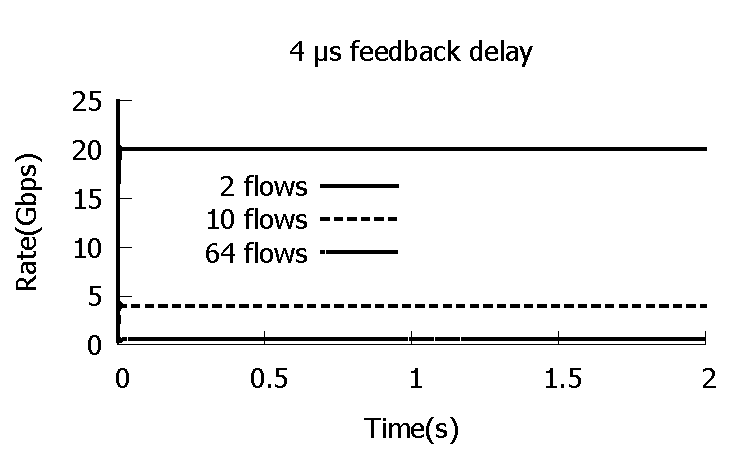
\includegraphics[width=0.49\columnwidth]{figures/stable_rate_4_pifixed.pdf}}
\subfigure[] {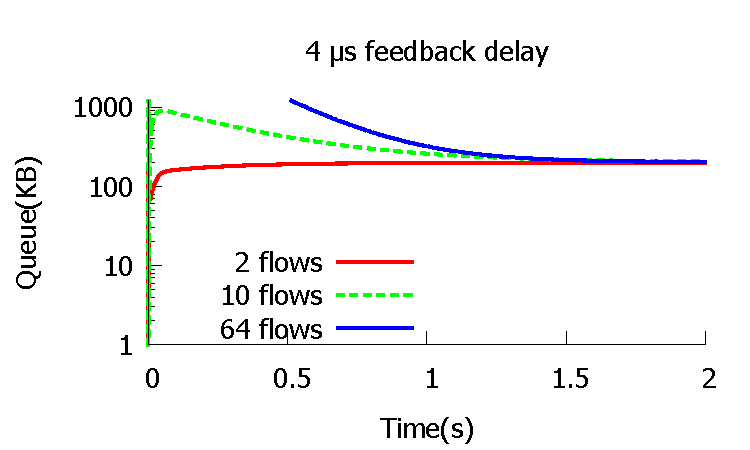
\includegraphics[width=0.49\columnwidth]{figures/stable_q_4_pifixed.pdf}}
\subfigure[] {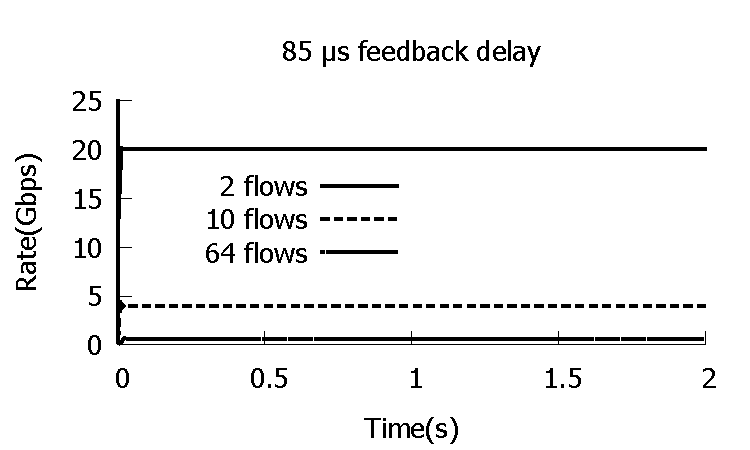
\includegraphics[width=0.49\columnwidth]{figures/stable_rate_85_pifixed.pdf}} 
\subfigure[] {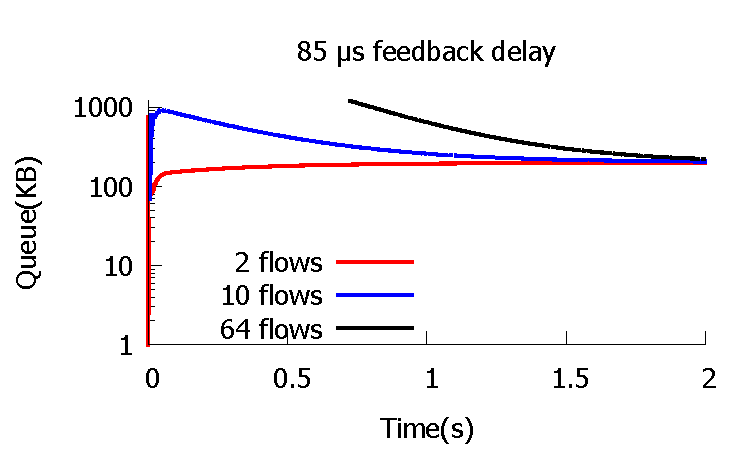
\includegraphics[width=0.49\columnwidth]{figures/stable_q_85_pifixed.pdf}}
\caption{DCQCN with PI controller}
\label{fig:dcqcn_pi}
\end{figure}

\fixme{TO DO}
In contrast, when we use a PI controller at the end hosts using delay
as the feedback signal, we see that although we can control the queue
to a specificed value, we cannot achieve fairness, as shown
in~Theorem~\ref{thm:fairness-delay}.
\begin{figure}
\center
%\includegraphics[width=0.33\textwidth]{figures/stable_timely_pi.pdf}
\caption{PI controller to stabilize TIMELY}
\label{fig:dcqcn_pi}
\end{figure}

%%% Local Variables:
%%% mode: latex
%%% TeX-master: "main"
%%% End:
